%\documentclass[12pt,a4paper]{article}
%\documentclass[12pt]{report}
\documentclass[a4paper,14pt]{report}
\usepackage[utf8]{inputenc}
\usepackage[14pt]{extsizes}
\usepackage{listings}
\usepackage{graphicx}
\graphicspath{{schemes/}}
\DeclareGraphicsExtensions{.pdf,.png,.jpg}
\usepackage[english,russian]{babel}
\usepackage{indentfirst}
\usepackage{pdfpages}
\usepackage{titlesec}
\usepackage{amsmath}
\usepackage{float}
\usepackage{caption}
\captionsetup{labelsep=endash}
\captionsetup[figure]{name={Рисунок}}
\newenvironment{comment}{}{}

% Для листинга кода:
\lstset{ %
basicstyle=\small\sffamily, % размер и начертание шрифта для подсветки кода
numbers=right,               % где поставить нумерацию строк (слева\справа)
numberstyle=\tiny,           % размер шрифта для номеров строк
stepnumber=1,                   % размер шага между двумя номерами строк
numbersep=5pt,                % как далеко отстоят номера строк от подсвечиваемого кода
showspaces=false,            % показывать или нет пробелы специальными отступами
showstringspaces=false,      % показывать или нет пробелы в строках
showtabs=false,             % показывать или нет табуляцию в строках
frame=single,              % рисовать рамку вокруг кода
tabsize=4,                 % размер табуляции по умолчанию равен 2 пробелам
captionpos=t,              % позиция заголовка вверху [t] или внизу [b]
breaklines=true,           % автоматически переносить строки (да\нет)
breakatwhitespace=false, % переносить строки только если есть пробел
escapeinside={\#*}{*)}   % если нужно добавить комментарии в коде
}

% Для измененных титулов глав:
\usepackage{titlesec, blindtext, color} % подключаем нужные пакеты
\definecolor{gray75}{gray}{0.75} % определяем цвет
\newcommand{\hsp}{\hspace{20pt}} % длина линии в 20pt
% titleformat определяет стиль
\titleformat{\chapter}[hang]{\Huge\bfseries}{\thechapter\hsp\textcolor{gray75}{|}\hsp}{0pt}{\Huge\bfseries}

%отступы по краям
\usepackage{geometry}
\geometry{verbose, a4paper,tmargin=2cm, bmargin=2cm, rmargin=1.5cm, lmargin = 3cm}
% межстрочный интервал
\usepackage{setspace}
\onehalfspacing
\usepackage{float}
% plot
\usepackage{pgfplots}
\usepackage{filecontents}
\usepackage{amsmath}
\usepackage{tikz,pgfplots}
\usetikzlibrary{datavisualization}
\usetikzlibrary{datavisualization.formats.functions}

\usepackage{graphicx}
\graphicspath{{src/}}
\DeclareGraphicsExtensions{.pdf,.png,.jpg}

\usepackage{indentfirst}
\setlength{\parindent}{1.4cm}
\usepackage{titlesec}
\titlespacing{\chapter}{0pt}{12pt plus 4pt minus 2pt}{0pt}
\renewcommand{\rmdefault}{ftm}
\begin{document}
\fontsize{14}{16pt}
\def\contentsname{Содержание}
%\def\chaptername{} % убирает "Глава"
%\includepdf[pages=1]{titul.pdf}

\tableofcontents

\newpage
\chapter*{Введение}
\addcontentsline{toc}{chapter}{Введение}
В настоящее время компьютерная графика является неотъемлемой частью компьютерных технологий. Она позволяет наглядно выводить данные, создавать удобные и красивые интерфейсы. Также компьютерная графика используется в компьютерных играх, и в кино для создания эффектов и трёхмерных сцен.

Чтобы сделать возможным корректное преобразование цифровых данных в графические необходимо решить задачи синтеза сцены.
 
Зачастую существует несколько алгоритмов способных решить ту или иную задачу. Каждый алгоритм имеет свои достоинства и недостатки, одни чуть быстрее, другие потребляют меньше ресурсов и так далее. На программиста ложится задача выбора алгоритма необходимого для конкретной ситуации.

Цель данной работы построить сцену, на которой присутствует модель топлива и реализовать моделирование эффекта горения, включающее визуализацию пламени и симуляцию распространения огня по поверхности модели.


Задачи данной лабораторной работы:
\begin{itemize}
 \item описать сцену и её элементы;
 \item проанализировать методы моделирования огня и выбрать метод, который будет использоваться в программе;
 \item проанализировать алгоритмы удаления невидимых граней и выбрать алгоритм, который будет использоваться в программе;
 \item проанализировать методы освещения и выбрать метод, который будет использоваться в программе;
 \item спроектировать и написать программное обеспечение;
 \item провести исследование написанного программного обеспечения.
\end{itemize}


\chapter{Аналитическая часть}
В данном разделе будут определены объекты сцены, рассмотрены и выбраны алгоритмы для синтеза сцены.

\section{Формализация объектов сцены} 
Сцена состоит из следующих объектов:
\begin{itemize}
\item модель топлива, данный объект состоят из плоских выпуклых многоугольников, образующих многогранник и задаются в виде точек, являющихся вершинами многоугольника и рёбер их соединяющих, каждая модель имеет свои параметры горения, температуры самовозгорания и цвета;
\item модель огня, данный объект состоит из точек генерации огня и частиц огня;
\item камера, данный объект задаёт положение наблюдателя и вектор его взгляда;
\item источник света, задаёт положение и интенсивность точечного источника света.
\end{itemize}

\section{Методы генерации пламени}
Существует два метода для генерации пламени:
\begin{itemize}
\item система частиц;
\item уравнения горячих газов.
\end{itemize}

\subsection{Система частиц}
Реалистичность и проработанность огня будет зависеть от количества частиц и от законов их поведения, однако с увеличением количества частиц алгоритм соответственно начнёт работать медленнее. С помощью данного метода можно визуализировать огонь, используя маленькие спрайты.
Пример использования системы частиц для моделирования огня изображён на рисунке \ref{fig:fire}.
\begin{figure}[H]
 \center{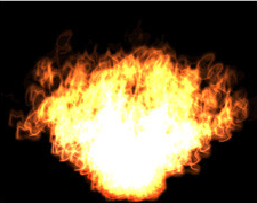
\includegraphics[scale = 1]{fire.png}}
 \caption{Система частиц огня}
 \label{fig:fire}
\end{figure}
\subsection{Уравнения горячих газов}
Данный метод полностью основан на физико-математическом подходе. В симуляции использовались несжатые уравнения Навье-Стокса для горячих газов, это позволило также смоделировать эффект расширения, вызванный испарением, и эффект текучести поднимающихся дыма и сажи. Однако данный подход сложно реализовать для работы в реальном времени, поскольку необходимо находить решение большого количества комплексных уравнений за время кадра. По этой причине данный способ не подходит.


Единственный подходящий метод, это система частиц, чтобы уменьшить их количество воспользуемся методом спрайтов, в таком случае на месте каждой частицы будет находится полупрозрачный спрайт из-за чего будет создаваться эффект пламени. Хотя данный подход и не даёт наиболее реалистичного пламени, он хорошо подходит для создания огня в режиме реального времени. Для реалистичного поведения пламени необходимо задать законы движения и взаимодействия его частиц. Для этого необходимо учитывать следующее:
\begin{itemize}
 \item тепловое расширения газа;
 \item закон Архимеда;
 \item сопротивление воздуха;
 \item тепловой обмен с окружающей средой \cite{fiz}.
\end{itemize}
\section{Алгоритм распространения огня}
Для распространения огня удобнее всего использовать систему точек генерации огня, производящую частички огня. Каждая точка такой системы имеет параметр температуры, который будет расти в зависимости от времени и материала модели.
При достижении некоторой температуры вокруг точки генерации огня на некотором расстоянии 
будут возникать новые точки, если они не были созданы до этого и лежат на модели.
 
\section{Анализ алгоритмов удаления невидимых линий и поверхностей}
Для корректного отображение модели топлива необходимо устранить невидимые рёбра. При выборе алгоритма удаления невидимых рёбер нужно учитывать скорость работы алгоритма, так как при медленной работе алгоритма динамическая анимация огня соответственно замедлится и поведение огня станет нереалистичным. Рассмотрим несколько алгоритмов.

\subsection{Алгоритм Робертса}
\par
Это метод основан на математическом подходе. Он работает в объектном пространстве, что является его плюсом. Алгоритм сперва удаляет рёбра, экранируемые самим телом. Затем каждое оставшееся ребро каждого тела сравнивается с каждым из оставшихся тел, таким образом определяется какие части рёбер экранируются. Так как происходит сравнение каждого тела с каждым, то вычислительная трудоёмкость будет зависеть от квадрата количества тел \cite{alg}. Времязатратность алгоритма Робертса при большом количестве тел, является его главным минусом.

\subsection{Алгоритм обратной трассировки лучей }
\par
Принцип обратной трассировки лучей состоит в том, что через каждую точку экрана как бы проводится обратный луч света до пересечения с ближайшим объектом сцены, далее из этой точки проводится луч в направлении источника света, таким образом, моделируется распространение света \cite{alg}.

Плюсом данного алгоритма является то, что он выполняет множество задач, с его помощью возможен расчет теней, также можно моделировать многократные отражения и преломления за счёт этого достигается высокая степень реалистичности.
Однако данный метод имеет множество недостатков, например, низкая скорость и высокая вычислительная стоимость расчетов из-за большого количества лучей для каждого из которых нужно вычислить пересечения.
Также алгоритм не предусматривает учёт вторичного освещения от диффузно отраженного объектами света.
Возникают резкие границы самих объектов и цветовых переходов тени, подсветки, прозрачности.

\subsection{Алгоритм Варнока}
\par
В отличие от алгоритма Робертса, алгоритм Варнока работает не в объектном пространстве, а в пространстве образа. Его главная идея заключается в том, чтобы на обработку тех областей, которые содержат мало информации тратилось мало времени и вычислений, а на области с высоким информационным содержимым тратилась большая вычислительная мощность. 
В пространстве изображения рассматривается окно и решается вопрос о том, пусто ли оно, или его содержимое достаточно просто для визуализации. Если это не так, то окно разбивается на фрагменты до тех пор, пока содержимое фрагмента не станет достаточно простым для визуализации или его размер не достигнет требуемого предела разрешения. 
Конкретная реализация алгоритма Варнока зависит от метода разбиения окна и от деталей критерия, используемого для того, чтобы решить, является ли содержимое окна достаточно простым. внешним, если он целиком находится вне окна \cite{alg}.

     Достоинством алгоритма Варнока можно назвать сравнительно низкую времязатратность, зависящую от эффективности разбиений количества многоугольников в кадре и необходимого разрешения. Однако из-за произвольной разбивки, выполняемой для распознавания, в изображениях возникают дефекты.


\subsection{Алгоритм Вейлера-Азертона} 
\par
    Данный алгоритм является оптимизацией алгоритма Варнока за счёт сокращения выполняемых разбиений, перейдя от прямоугольных разбиений к разбиениям вдоль границ многоугольников.

Для оптимизации в алгоритм были добавлены пункты:
\begin{itemize}
\item предварительная сортировка по глубине;

\item отсечение по границе ближайшего к точке наблюдения многоугольника, называемое сортировкой многоугольников на плоскости;

\item удаление многоугольников, экранируемых более близкими к точке наблюдения многоугольниками.

\end{itemize}
    Эффективность такого метода, как и алгоритм Варнока, зависит от эффективности разбиений и точно также, как и в алгоритме Варнока при построении изображения возникают дефекты \cite{alg2}.
  
\subsection{Метод Z-буфера}
\par
Этот алгоритм работает в пространстве изображения. Главным преимуществом алгоритма является его простота. Кроме того, этот алгоритм делает тривиальной визуализацию пересечений сложных поверхностей. Сцены могут быть любой сложности. Поскольку габариты пространства изображения фиксированы, оценка вычислительной трудоемкости алгоритма не более чем линейна. Элементы сцены не нужно предварительно сортировать по приоритету глубины. За счёт этого экономится вычислительное время, затрачиваемое на сортировку по глубине \cite{alg}.
Недостатком алгоритма является большой объем требуемой памяти, однако при современных технологиях это не является проблемой, а также можно использовать z-буфер с сканирующей строкой, что уменьшит необходимую память. 
Другой недостаток алгоритма состоит в трудоемкости реализации эффектов, связанных с полупрозрачностью, и ряда других специальных задач, повышающих реалистичность изображения, однако в моей работе это и не требуется. 


  Хотя метод обратной трассировки лучей и является наиболее подходящим так как обеспечивает одновременно удаление невидимых поверхностей и создание реалистичного света, его времязатратность не даёт возможности воспроизводить анимацию огня в реальном времени без больших вычислительных мощностей. Наилучшим образом тут подойдёт алгоритм Z- буфера. Данный алгоритм будет самым быстро действенным из всех перечисленных, простым в реализации и создающим малое количество дефектов изображения.

\section{Перевод точки в экранные координаты}
Для отображения модели на экране необходимо перевести координаты её точек из объектных в экранные.
Предполагается, что камера находится в нуле координат и вектор взгляда совпадает с осью z. 
В таком случае нам необходимо в начале применить к точкам преобразования для перевода их в пространство камеры.
После того как все преобразования сделаны необходимо отмасштабировать x и y пропорционально их удалённости по оси z и в зависимости от угла обзора камеры, это демонстрируется на рисунках \ref{fig:geom1}, \ref{fig:geom2}; 
\begin{figure}[H]
 \center{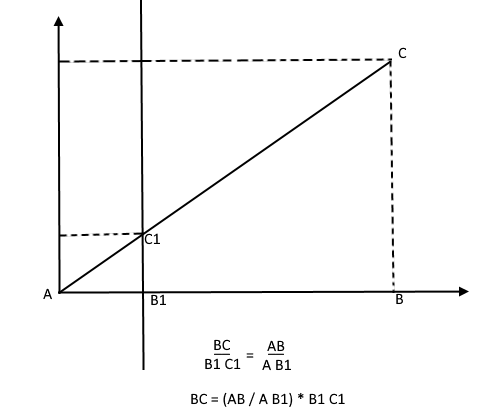
\includegraphics[scale = 1]{4.png}}
 \caption{Геометрия преобразований 1}
 \label{fig:geom1}
\end{figure}

\begin{figure}[H]
 \center{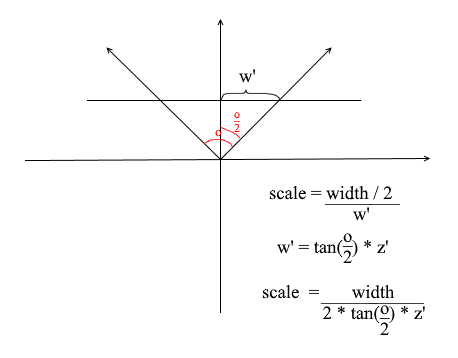
\includegraphics[scale = 1]{3.png}}
 \caption{Геометрия преобразований 2}
 \label{fig:geom2}
\end{figure}
Получим формулы \ref{eq10:ref}, \ref{eq9:ref} преобразования координат x и y.
\begin{equation}
 x' = x / (z + 1) * scale
 \label{eq10:ref}                  
 \end{equation}                                                                                              
 \begin{equation}
   y' = y / (z + 1) * scale
 \label{eq9:ref}                  
 \end{equation}                                                                                              
\section{Преобразования}
Для изменения сцены необходимо реализовать простейшие преобразования над объектами, такие как сдвиг, и поворот. Для этих целей будут использоваться формулы \ref{eq5:ref}, \ref{eq6:ref}, \ref{eq7:ref}, \ref{eq8:ref}.

Сдвиг:
\begin{equation}
\begin{cases}
 X=X+Dx,
 \\
 Y=Y+Dy,
 \\
 Z=Z+Dz.  
\end{cases}
 \label{eq8:ref}                  
 \end{equation}                                                                                              
Поворот вокруг:
\newline
    OX:
    \begin{equation}
    \begin{cases}
  z'= -y*sin(ax)+z*cos(ax),
  \\
  x'= x,
  \\
  y'= y*cos(ax)+z*sin(ax).
 \end{cases}
 \label{eq7:ref}                  
 \end{equation}                                                                 
    OY:
    \begin{equation}
    \begin{cases}
  z'= -x*sin(ay)+z*cos(ay),
  \\
  x'= x*cos(ay)+z*sin(ay),
  \\
  y'= y.
 \end{cases}
 \label{eq6:ref}                  
 \end{equation} 
    OZ:
    \begin{equation}
    \begin{cases}
  z'= z,
  \\
  x'= x*cos(az)-y*sin(az),
  \\                                                             
  y'= x*sin(az)+y*cos(az).  
 \end{cases}                                                              
 \label{eq5:ref}                  
 \end{equation} 

\section{Освещение}
Для того чтобы объекты сцены было видно, и они выглядели объёмно, на сцене должно присутствовать освещение.
Существует три компоненты освещения:
\begin{itemize}
\item фоновое;
\item рассеяное;
\item зеркальное.
\end{itemize}


Фоновое освещение. Данный вид освещения используется для того чтобы сцена не была тёмной. За счёт данного освещения объекты не будут абсолютно чёрными и будут видны его очертания. Чтобы имитировать это, используем некоторую константу освещения, которая всегда будет придавать объекту некоторый оттенок, данная константа должна быть сравнительно небольшой, чтобы не сильно перебивать другие виды освещений.
\begin{equation}
Ia = ka * ia ,
\label{eq4:ref}                  
\end{equation}                                             
где

$Ia$ – фоновая составляющая освещенности в точке;

$ka$ – свойство материала воспринимать фоновое освещение;

$ia$ – мощность фонового освещения.


Диффузное освещение имитирует воздействие на объект направленного источника света. Это наиболее визуально значимый компонент модели освещения. Чем большая часть поверхности объекта обращена к источнику света, тем ярче он будет освещен.
\begin{equation}
I_d=K\_d* i\_d*(\vec{L} * \vec{N}),  
\label{eq3:ref}                  
\end{equation}                                 
где

$Id$– рассеянная составляющая освещенности в точке;

$kd$– свойство материала воспринимать рассеянное освещение;

$id$– мощность рассеянного освещения;

$L$ – направление из точки на источник;

$N$ - вектор нормали в точке.


Освещение зеркальных бликов - это яркие пятна света или блик. По цвету зеркальные блики часто ближе к цвету источника света, чем к цвету объекта. Яркость и размер бликов зависят от того, насколько гладкая поверхность \cite{alg2}.
     Поверхности объектов будут однотонными, следовательно, будут иметь свои показатели поглощения и отражения цветов.
     Формула для вычисления зеркальных бликов выглядит следующим образом:
\begin{equation}
I_s=K\_s* i\_s*[(\vec{V} * \vec{R} )]^a, 
\label{eq2:ref}                  
\end{equation} 
 где

$Is$ – зеркальная составляющая освещенности в точке;

$ks$ – коэффициент зеркального отражения;

$is$ – мощность зеркального освещения;

$R$ – направление отраженного луча;

$V$ - направление на наблюдателя;

$a$ - коэффициент блеска, свойство материала;

\subsection{Метод Фонга и метод Гуро.}
Для вычисления зеркалного и рассеянного света существует два подхода:
\begin{itemize}
 \item метод Гуро обеспечивает непрерывность освещенности за счет ее билинейной интерполяции: после определения значений освещенности в вершинах полигона применяют линейную интерполяцию вдоль сторон полигона, а потом – линейную интерполяцию между сторонами полигона вдоль каждой из сканирующих строк, пересекающих полигон (при этом освещенность рассчитывается для каждого пикселя соответствующего интервала сканирующей строки);
    \item метод Фонга аналогичен методу Гуро, но при его использовании для определения цвета в каждой точке интерполируются не интенсивности отраженного света, а векторы нормалей.
\end{itemize}
    Метод Фонга требует больше вычислений, чем метод Гуро, однако даёт гораздо лучшее качество изображения рисунок \ref{fig:fong}.
    \begin{figure}[H]
 \center{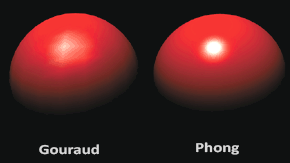
\includegraphics[scale = 1]{1.png}}
 \caption{Закраска по Фонгу и Гуро}
 \label{fig:fong}
\end{figure}
    
                              

\subsection{Простая закраска}
Данный вид закраски подразумевает только вычисления цвета по формуле без необходимости интерполяции интенсивности или вектора нормали.
Поскольку в данном случае используется модель с плоскими гранями, то интерполяция цвета не требуется, поэтому будем применять простую закраску.


Общая формула \ref{eq1:ref} для закраски будет суммой формул \ref{eq2:ref},\ref{eq3:ref}, \ref{eq4:ref} поделённой на квадрат расстояния до источника света:
\begin{equation}
I= ka • ia +  (K\_d* i\_d*(\vec{L} * \vec{N} )+ K\_s* i\_s*([\vec{V} * \vec{R}]^a)/(d^2)   
\label{eq1:ref}                  
\end{equation}
Интерполяция вектора нормали производится не будет.

\section*{Вывод из аналитической части}
\addcontentsline{toc}{section}{Вывод из аналитической части}
В данном разделе были рассмотрены алгоритмы удаления невидимых линий и поверхностей, методы освещения и моделирования огня. В качестве алгоритма удаления невидимых линий был выбран Z-буфер, для моделирования огня была выбрана система частиц с наложением на них спрайтов, в качестве метода затенения был выбран простой алгоритм.

\chapter{Конструкторская часть}
В данном разделе будут рассмотрены требования к программе и
алгоритмы, используемые в программе.


\section{Требования к программе}
Программа должна предоставлять следующие возможности:
\begin{itemize}
\item визуальное отображение сцены;
\item добавление нового очага возгорания в сцену;
\item выбор материала модели из набора (дерево, древесный уголь, каменный уголь, торф);
\item задать положение и интенсивность точечного источника света;
\item перемещение камеры по сцене и поворот камеры по вертикали и горизонтали.
\end{itemize}
\section{Схема взаимодействия классов}
На рисунках \ref{fig:class1}, \ref{fig:class2}, \ref{fig:class3} приведены UML диаграммы взаимодействия классов.

\begin{figure}[H]
 \center{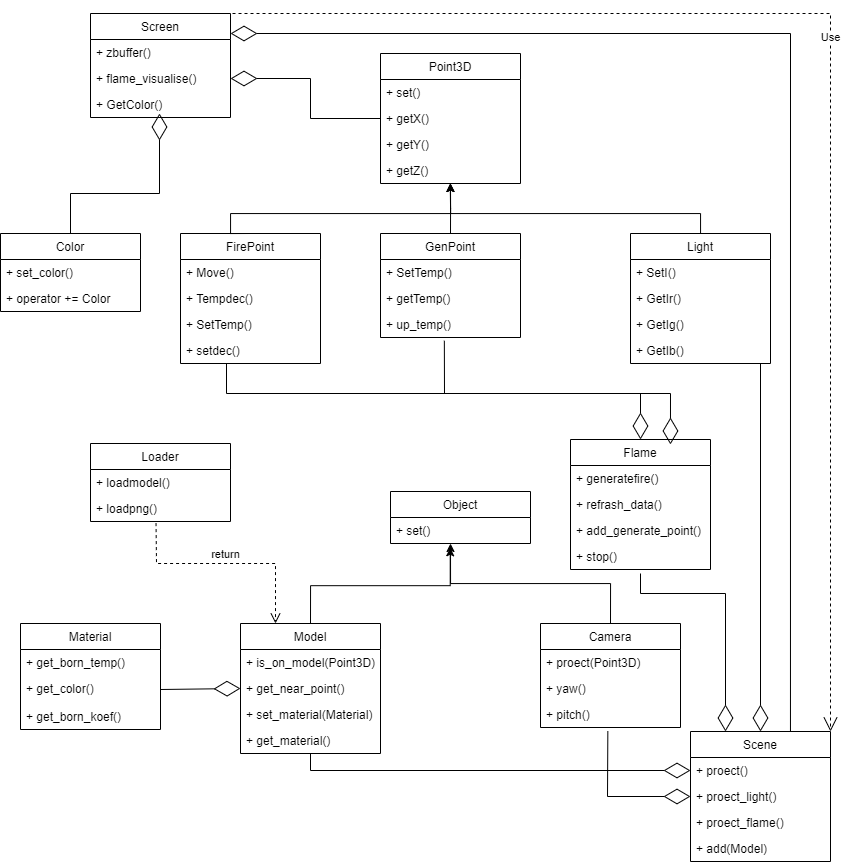
\includegraphics[scale = 0.5]{UML.png}}
 \caption{UML Диаграма часть 1}
 \label{fig:class1}
\end{figure}

\begin{figure}[H]
 \center{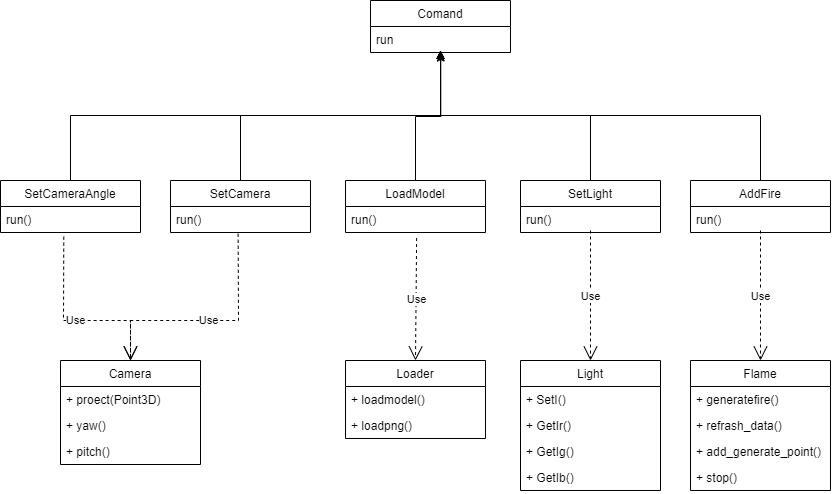
\includegraphics[scale = 0.5]{UML2.png}}
 \caption{UML Диаграма часть 2}
 \label{fig:class2}
\end{figure}

\begin{figure}[H]
 \center{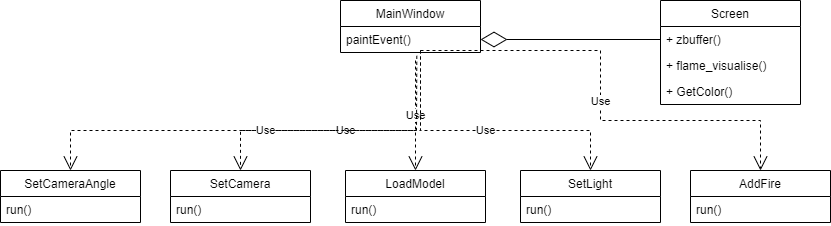
\includegraphics[scale = 0.5]{UML3.png}}
 \caption{UML Диаграма часть 3}
 \label{fig:class3}
\end{figure}
\section{Описание алгоритмов}
Далее приведены схемы алгоритмов для создания программного обеспечения.
\subsection{Основной алгоритм}
На рисунке \ref{fig:sh1} приведена схема основного алгоритма.
\begin{figure}[H]
 \center{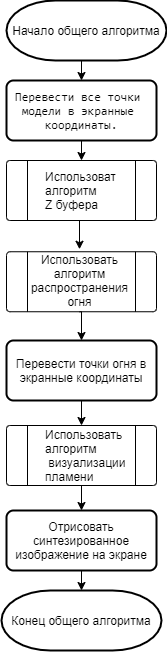
\includegraphics[scale = 0.8]{Main.png}}
 \caption{Схема основного алгоритма}
 \label{fig:sh1}
\end{figure}
\subsection{Алгоритм Z-буффера}
На рисунках 2.5, \ref{fig:sht2} приведена схема алгоритма Z-буффера.
 \begin{figure}[H]
 \center{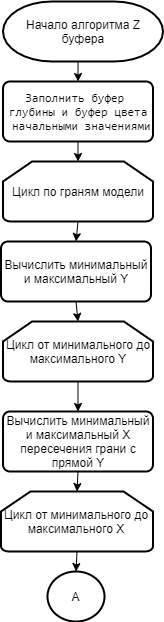
\includegraphics[scale = 0.8]{Zbuf1.png}}
 \caption{Схема алгоритма Z-буфера часть 1}
 \label{fig:sh2}
\end{figure}
\begin{figure}[H]
 \center{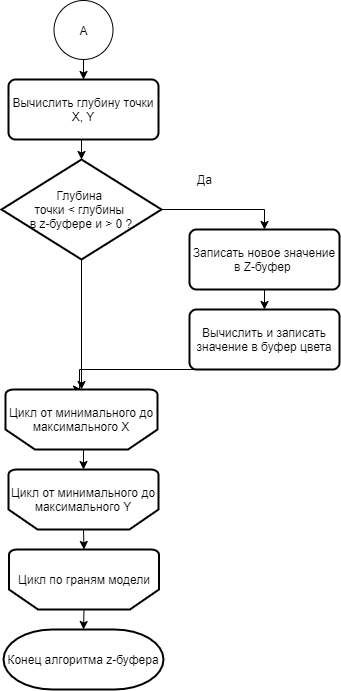
\includegraphics[scale = 0.8]{Zbuf2.png}}
 \caption{Схема алгоритма Z-буфера часть 2}
 \label{fig:sht2}
\end{figure}
\subsection{Алгоритм моделирования огня}
На рисунке \ref{fig:sh3} приведена схема алгоритма моделирования огня.
\begin{figure}[H]
 \center{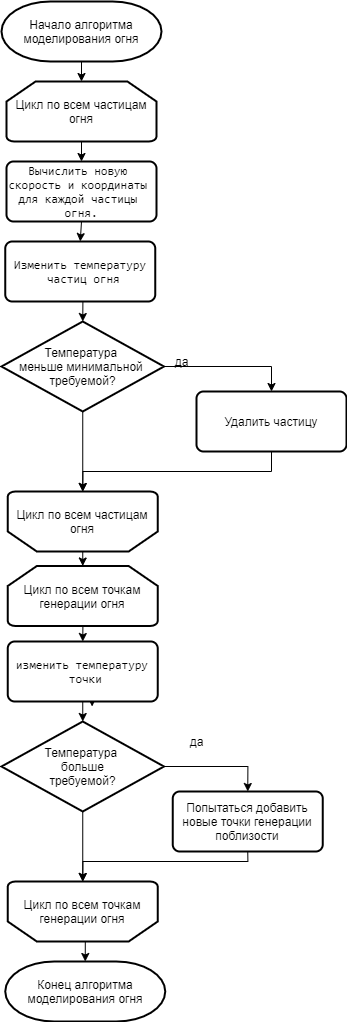
\includegraphics[scale = 0.7]{Renew.png}}
 \caption{Схема алгоритма моделирования огня}
 \label{fig:sh3}
\end{figure}
\subsection{Алгоритм визуализации огня}
На рисунке \ref{fig:sh4} приведена схема алгоритма визуализации огня.
\begin{figure}[H]
 \center{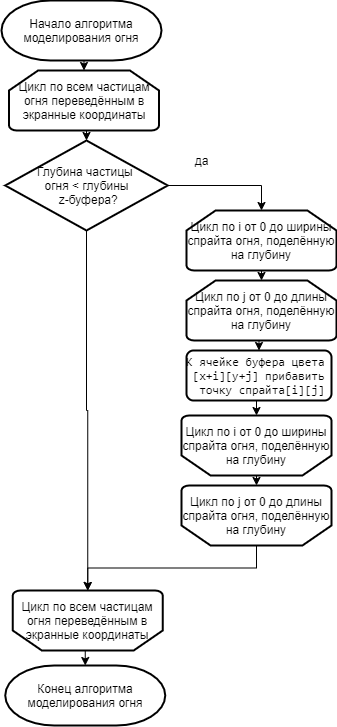
\includegraphics[scale = 0.7]{Visual.png}}
 \caption{Схема алгоритма визуализации огня}
 \label{fig:sh4}
\end{figure}
\section{Распараллеливание задач}
Если сделать последовательным выполнение вычислений и отрисовки, это приведёт к зависанию приложения так как основной поток будет занят циклом вычислений и не сможет откликаться на команды пользователя.
Поэтому для выполнения вычислений создаётся отдельный поток, который при окончании вычислений будет вызывать событие отрисовки в главном потоке. 
В таком случае для корректной отрисовки буфера цвета необходимо, чтобы поток выполняющий вычисления дожидался окончания отрисовки. Для этого будет использоваться мьютекс.
\section{Модель горючего материала}
Для демонстрации работы программы была выбрана модель кубика с вершинами в точках , представленных в таблице 2.1, данный выбор обусловлен удобством данной модели для установки точки горения и наблюдения за распространением огня. Пользователь может задавать тип материала модели, однако форма и размеры модели будут оставаться неизменными.

\begin{table}[h]
\label{tab:toc} 
\caption{Координаты точек куба}
\begin{center}
\begin{tabular}{ | c | c | c | c |}
\hline
№ точки & координата x & координата y & координата z \\ \hline
1 & 1 & 1 & 1 \\
2 & -1 & 1 & 1 \\
3 & 1 & -1 & 1\\
4 & -1 & -1 & 1\\
5 & 1 & 1 & -1 \\
6 & -1 & 1 & -1 \\
7 & 1 & -1 & -1\\
8 & -1 & -1 & -1\\
\hline
\end{tabular}
\end{center}
\end{table}

\section*{Вывод из конструкторской части}
\addcontentsline{toc}{section}{Вывод из конструкторской части}
В данном разделе были приведены алгоритмы для создания программного обеспечения, рассмотрены схемы взаимодействия классов, приведены схемы алгоритмов.
Был сделан вывод о необходимости распараллеливания задач.

\chapter{Технологическая часть}
В данном разделе рассматриваются, производится выбор средств реализации, рассматривается строение программного обеспечения.

\section{Средства реализации}
В качестве языка программирования был выбран C++ по следующим причинам:
\begin{itemize}
\item имеется опыт программирования на это языке, что сократит время написания и отладки программы;
\item данный язык предоставляет возможность объектно-ориентированного программирования, что позволяет рассматривать элементы сцены как объекты, это сделает взаимодействие между элементами сцены более понятными и удобными для разработчика;
\item для данного языка имеется множество библиотек.
\end{itemize}

В качестве среды разработки была выбрана «QT Creator» по следующим причинам:
\begin{itemize}
\item данная среда разработки бесплатна в пользовании студентами;
\item она имеет множество удобств, которые облегчают процесс написания и отладки кода;
\item имеется опыт работы в данной средой разработки, что сократит время изучения возможностей среды. 
\end{itemize}

\section{Структура приложения}
Приложение состоит из следующих модулей:
\begin{itemize}
 \item INCLUDS.h - файл подключения основных библиотек и определений;
    \item Objects.h - файл определения классов;
    \item Primitiv.h - файл определения классов;
    \item algoritms.h - файл определения классов;
    \item comands.h - файл определения классов;
    \item loader.h - файл определения классов;
    \item mainwindow.h - файл определения классов;
    \item mutexs.h - файл определения классов;
    \item screen.h - файл определения классов;
    \item mainwindow.ui - файл содержащий дизайн интерфейса;
    \item alghoritms.cpp - файл функций классов;
    \item comands.cpp - файл функций классов;
    \item loader.cpp - файл функций классов;
    \item main.cpp - файл содержавший функцию main();
    \item mainwindow.cpp - файл функций классов;
    \item object.cpp - файл функций классов;
    \item primitiv.cpp - файл функций классов;
    \item screen.cpp - файл функций классов.
\end{itemize}

Также в директории с исполняемым файлом находятся следующие файлы:
\begin{itemize}
 \item coub.obj - Файл содержащий описание модели в формате obj;
 \item fire0.bmp - 24 битный bmp файл содержащий спрайт частиц огня.
\end{itemize}
\section{Интерфейс приложения}
На рисунке \ref{fig:inter} изображён интерфейс приложения.
\begin{figure}[H]
 \center{\includegraphics[scale = 0.7]{interface.png}}
 \caption{Интерфейс приложения}
 \label{fig:inter}
\end{figure}
Интерфейс поделён на 4 логические части расположенных на форме:
\begin{itemize}
\item камера;
\begin{itemize}
\item поле "X" задаёт координату x камеры в виде числа с десятичной дробью;
\item поле "Y" задаёт координату y камеры в виде числа с десятичной дробью;
\item поле "Z" задаёт координату z камеры в виде числа с десятичной дробью;
\item поле "Угол вертикального поворота камеры" задаёт вертикальный наклон камеры в градусах в виде числа с десятичной дробью;
\item поле "Угол горизонтального поворота камеры" задаёт поворот камеры по оси OY в градусах в виде числа с десятичной дробью;
\item кнопка "Переместить камеру", при корректном заполнении полей "X", "Y", "Z", переносит камеру в координаты, введённые в полях "X", "Y", "Z";
\item кнопка "Повернуть камеру", при корректном заполнении полей "Угол вертикального поворота камеры", "Угол горизонтального поворота камеры", задаёт углы поворота камеры, введённые в полях "Угол вертикального поворота камеры", "Угол горизонтального поворота камеры";
\end{itemize}
\item модель;
\begin{itemize}
\item в окошке с выбором можно выбрать тип материала модели из набора (дерево, каменный уголь, древесный уголь, торф);
\item кнопка "Установить модель" меняет материал модели на выбранный, при этом все точки распространения огня, присутствующие на модели удаляются;
\end{itemize}
\item источник света;
\begin{itemize}
\item поле "X" задаёт координату x источника света в виде числа с десятичной дробью;
\item поле "Y" задаёт координату y источника света в виде числа с десятичной дробью;
\item поле "Z" задаёт координату z источника света в виде числа с десятичной дробью;
\item поле "IR" задаёт интенсивность красной составляющей цвета источника света в виде целого числа;
\item поле "IG" задаёт интенсивность зелёной составляющей цвета источника света в виде целого числа;
\item поле "IB" задаёт интенсивность синей составляющей цвета источника света в виде целого числа;
\item кнопка "Установить источник света", при корректном заполнении полей "X", "Y", "Z", "IR", "IG", "IB", переносит источник света в координаты введённые в полях "X", "Y", "Z", и задаёт его интенсивность, введённую в полях "IR", "IG", "IB";
\end{itemize}
\item точка распространения огня;
\begin{itemize}
\item поле "X" задаёт координату x точки распространения в виде числа с десятичной дробью;
\item поле "Y" задаёт координату y точки распространения в виде числа с десятичной дробью;
\item поле "Z" задаёт координату z точки распространения в виде числа с десятичной дробью;
\item кнопка "Добавить точку распространения огня", при корректном заполнении полей "X", "Y", "Z" и при условии, что тока с соответствующими координатами принадлежит поверхности модели.
\end{itemize}
\end{itemize}
Начиная от верхнего левого угла на форме расположен экран размером 600 X 400 на который выводится синтезированное изображение.
\section{Листинги алгортмов программы}
В листингах 3.1 - 3.6 приведены реализации основных алгоритмов, используемых в программе.
\newpage
\begin{center}
\captionsetup{justification=raggedright,singlelinecheck=off}
\begin{lstlisting}[language=C++,
                   directivestyle={\color{black}}
                   emph={int,char,double,float,unsigned},
                   emphstyle={\color{blue}}, caption = Функция Z-буфера часть 1] 
void Screen::zbuffer(std::vector <Model> &m)
{
    std::vector <List> edges = m[0].edges;
    int addnum = -1;
    int ystart, yend, xfirst, xlast, buf, intersect;
    std::vector <int> intersections;
    Point3D K, N;
    double CalcZ;
    fill(Zbuf, Cbuf);
    for(int l = 0; l < edges.size(); l++)
    {
    K = CalcKoef(edges[l], P, addnum);
    N = Normal(edges[l], P, addnum);
    MinMaxY(edges[l], P, ystart, yend, addnum);
    for (int y = ystart; y <= yend; y++)
    {
        edges[l].to_end();
        buf = edges[l].get_npoint() + addnum;
        for (edges[l].to_begin();!edges[l].is_end(); edges[l].next())
        {
            intersect = intersection(P[buf].getX(),P[buf].getY(),P[edges[l].get_npoint()+addnum].getX(),P[edges[l].get_npoint()+addnum].getY(), y);
            buf = edges[l].get_npoint() + addnum;
            if (intersect != -1)
                intersections.push_back(intersect);
        }
\end{lstlisting}
\newpage
\begin{lstlisting}[language=C++,
                   directivestyle={\color{black}}
                   emph={int,char,double,float,unsigned},
                   emphstyle={\color{blue}}, caption = Функция Z-буфера часть 2] 
        intersect = intersection(P[buf].getX(),P[buf].getY(),P[edges[l].get_npoint()+addnum].getX(),P[edges[l].get_npoint()+addnum].getY(), y);
        if (intersect != -1)
            intersections.push_back(intersect);
        if (intersections.size() < 2)
            continue;
        MinMaxX(intersections, xfirst, xlast);
        intersections.clear();
        for (int x = xfirst; x <= xlast; x++)
        {
            CalcZ = x*K.getX() + y*K.getY() + K.getZ();
            if (Zbuf[x][y] > CalcZ and CalcZ > 0)
            {
                Zbuf[x][y] = CalcZ;
                Point3D P0((x - WINWIDTHD2) * ((CalcZ + 1 > EPS) ? (CalcZ + 1) : 0.001) / MKOEF, (y - WINHEIGHTD2) * ((CalcZ + 1 > EPS) ? (CalcZ + 1) : 0.001) / MKOEF, CalcZ);
                Cbuf[x][y] = pixelcolor(m[0].mat.get_color(), P0, N, Lights);
            }
        }
    }
    }
}
\end{lstlisting}
\end{center}
\newpage
\begin{center}
\captionsetup{justification=raggedright,singlelinecheck=off}
\begin{lstlisting}[language=C++,
                   directivestyle={\color{black}}
                   emph={int,char,double,float,unsigned},
                   emphstyle={\color{blue}},label=brute,caption = Функция визуализации огня]
void Screen::flame_visualise()
{
    double x, y, z;
    double e;
    for (Point3D P : Flame)
    {
        x = P.getX();
        y = P.getY();
        z = P.getZ();
        double K = z*FKOEF;
        int maxx = round(flame_mask.size()/K);
        int maxy;
        if (maxx > 0)
            maxy = round(flame_mask[0].size()/K);
        int maxxd2 = maxx / 2;
        if (x > -maxx and x < WINWIDTH + maxx and y > -maxy and y < WINHEIGHT + maxy and abs(z) > 0.5)
            for(int i = 0; i < maxx and (x+i-maxxd2)>0 and (x+i-maxxd2)<WINWIDTH; i++)
            {
               int maxyd2 = maxy / 2;
               for(int j = 0; j < maxy and (y+j-maxyd2)>0 and (y+j-maxyd2)<WINWIDTH; j++)
               {
                   if (Zbuf[x+i-maxxd2][y+j-maxyd2] >= z)
                        Cbuf[x+i-maxxd2][y+j-maxyd2] += flame_mask[i*K][j*K];
               }
            }
    }
}
\end{lstlisting}
\end{center}
\newpage
\begin{center}
\captionsetup{justification=raggedright,singlelinecheck=off}
\begin{lstlisting}[language=C++,
                   directivestyle={\color{black}}
                   emph={int,char,double,float,unsigned},
                   emphstyle={\color{blue}},label=brute,caption = Функция обновления данных частиц огня]

void Flame::refrash_data()
{
    if (fire.size() == 0)
        return;
    int envtemp = MinTemp;
    long long sr = 0;
    int ch = 0;
    double dist = 0;
    std::list <FirePoint> :: iterator it = fire.begin();
    for (;it!=fire.end();it++)
    {
        sr = 0;
        ch = 0;
        for (FirePoint &F: fire)
        {
            dist = F.sqrdistP(*it);
            if (dist > EPS and dist < 0.01)
            {
                sr += F.GetT();
                ch++;
                if (ch == 10)
                    break;
            }
        }
        for (int i = ch; i < 10; i++)
        {
            sr += MinTemp;
            ch++;
        }
        it->setdec(sr/ch);
        it->Tempdec();
        if (it->GetT() < MinTemp or it->get_speed() < EPS)
            fire.erase(it);
        else
            it->Move();
    }
    for (int i = 0; i < (5 - (fire.size()/generate.size())) ; i++)
        generatefire();
};
\end{lstlisting}
\end{center}
\newpage
\begin{center}
\captionsetup{justification=raggedright,singlelinecheck=off}
\begin{lstlisting}[language=C++,
                   directivestyle={\color{black}}
                   emph={int,char,double,float,unsigned},
                   emphstyle={\color{blue}},label=brute,caption = Цикл работы] 
void actionThread(thr data)
{
    while(true)
    {
     comand_mtx.lock();
     data.scene.proect(data.Points);
     data.scene.proect_light(data.light);
     data.scene.proect_flame(data.FlameP);
     data.flame.refrash_data();
     data.flame.check_genpoints(data.model[0]);
     comand_mtx.unlock();
     draw_mtx.lock();
     data.screen.zbuffer(data.model);
     data.screen.flame_visualise();
     draw_mtx.unlock();
     data.m.update();
    }

}
\end{lstlisting}
\end{center}
\newpage
\begin{center}
\captionsetup{justification=raggedright,singlelinecheck=off}
\begin{lstlisting}[language=C++,
                   directivestyle={\color{black}}
                   emph={int,char,double,float,unsigned},
                   emphstyle={\color{blue}},label=brute,caption = Функция перевода точки в экранный координаты] 
Point3D Camera::proect(Point3D &P)
{
    double sx = P.getX() - position.getX();
    double sy = P.getY() - position.getY();
    double sz = P.getZ() - position.getZ();
    double x = sx * cosY + sz * sinY;
    double y = sy;
    double z = sz * cosY - sx * sinY;
    sx = x;
    sy = y * cosX + z * sinX;
    sz = z * cosX - y * sinX;
    x = sx * cosZ - sy * sinZ;
    y = sy * cosZ - sx * sinZ;
    if (sz + 1 > EPS)
    {
        x = x * MKOEF / (sz + 1)  + WINWIDTHD2;
        y = y * MKOEF / (sz + 1) + WINHEIGHTD2;
    }
    else
    {
        x = x * MKOEF * 1000 + WINWIDTHD2;
        y = y * MKOEF * 1000 + WINHEIGHTD2;
    }
    return Point3D(x , y , sz);
}
\end{lstlisting}
\end{center}
\section*{Вывод из технической части}
\addcontentsline{toc}{section}{Вывод из технической части}
В данном разделе были рассмотрены основные сведения о модулях программного обеспечения. Приводятся листинги реализаций алгоритмов. 

\chapter{Исследовательская часть}
В данном разделе будет проведены исследования программы, и проведен анализ полученных данных.
Все эксперименты проводились на машине со следующими характеристиками:
\begin{itemize}
 \item операционная система: Windows 10 64-разрядная операционная система;
 \item процессор: Intel(R) Core(TM) i3-7020U CPU @ 2.30GHz;
 \item оперативная память: 8,00 ГБ.
\end{itemize}
\section{Первое исследование}
Проведём исследование: как количество частичек огня в системе повлияет на производительность программы.
Для этого для количества частиц огня от 0 до 2000 с шагом 100 замерим время одного рабочего цикла программы. 
Для повышения точности, измерения будут проводится несколько раз. В качестве результата возьмём среднее арифметическое всех замеров. Также, для наглядной оценки по данным эксперимента составим график зависимости время одного рабочего цикла от количества частиц огня.

\section{Результаты первого исследования}
Результаты замеров времени внесены в таблицу 4.1 и визуализированы на графике, рисунок \ref{gra:ref1}.
\newline

\begin{table}[h]
\caption{Результаты первого эксперимента}
\label{table:res1} 
\begin{center}
\begin{tabular}{ | c | c | }
\hline
Количество частиц & Время мс.  \\ \hline
0 & 100 \\
100 & 101 \\
200 & 107 \\
300 & 115 \\
400 & 120 \\
500 & 124 \\
600 & 130 \\
700 & 135 \\
800 & 150 \\
900 & 156 \\
1000 & 160 \\
1100 & 166 \\
1200 & 173 \\
1300 & 180 \\
1400 & 185 \\
1500 & 194 \\
1600 & 202 \\
1700 & 211 \\
1800 & 217 \\
1900 & 221 \\
2000 & 230 \\
\hline
\end{tabular}
\end{center}
\end{table}


\begin{center}
\begin{figure}[H]
\begin{tikzpicture}[scale=1.2]
\begin{axis}[
 title = Зависимость времени работы от кол-ва частиц огня,
 xlabel = {$x$},
 ylabel = {$y$, мс},
 minor tick num = 2
]
\addplot coordinates {
(0 , 100) (100 , 101 )
(200 , 107 )
(300 , 115 )
(400 , 120 )
(500 , 124 )
(600 , 130 )
(700 , 135 )
(800 , 150 )
(900 , 156 )
(1000 , 160 )
(1100 , 166 )
(1200 , 173)
(1300 , 180)
(1400 , 185 )
(1500 , 194 )
(1600 , 202 )
(1700 , 211 )
(1800 , 217 )
(1900 , 221 )
(2000 , 230 )
};
\end{axis}
\end{tikzpicture}
\caption{График зависимости времени работы одного прохода цикла от количества частиц огня}
 \label{gra:ref1}
\end{figure}
\end{center}

\section{Второе исследование}
Проведём исследование: влияет ли тип модели топлива на скорость распространения огня.
Для этого замерим время, прошедшее от задания пользователем первой точки до появления на модели 100 точек генерации огня. Для наибольшей точности проведём замеры по 3 раза.

\section{Результаты второго исследования}
Результаты замеров времени внесены в таблицу \ref{tab:ref2}.
\newline

\begin{table}[h]
\label{tab:ref2} 
\caption{Результаты второго эксперимента}
\begin{center}
\begin{tabular}{ | c | c | c | c |}
\hline
Тип материала & 1 Замер мс. & 2 Замер мс. & 3 Замер мс. \\ \hline
Дерево & 61290 & 67126 & 59149 \\
Каменный уголь & 34630 & 36089 & 39670 \\
Древесный уголь & 26062 & 26574 & 28940\\
Торф & 52933 & 53155 & 54902\\
\hline
\end{tabular}
\end{center}
\end{table}
\section*{Вывод из исследовательской части}
\addcontentsline{toc}{section}{Вывод из исследовательской части}
По результатам проведённых исследований можно сделать следующие выводы:
\begin{itemize}
\item зависимость времени одного цикла алгоритма от количества частиц огня линейная;
\item тип модели влияет на скорость распространения пламени.

\end{itemize}


\chapter*{Заключение}
\addcontentsline{toc}{chapter}{Заключение}
В результате выполнения курсовой работы были выполнены все поставленные задачи. Было разработано и написано программное обеспечение.
Были проведены исследования зависимости времени отрисовки от количества частиц огня и проверена зависимость скорости распространения огня от типа материала. По результатам исследований были сделаны выводы, что
зависимость времени одного цикла алгоритма от количества частиц огня линейная и
тип модели влияет на скорость распространения пламени.
 
\addcontentsline{toc}{chapter}{Список литературы}
\begin{thebibliography}{6}
\bibitem{alg} D. F. Rogers. Procedural Elements for Computer Graphics. 2nd ed., 1998 – p.457-517 
\bibitem{alg2} Никулин, Е.А. Компьютерная графика. Модели и алгоритмы: Учебное пособие / Е.А. Никулин. - СПб.: Лань, 2018. - 708 c.
\bibitem{} Шикин Е.В., Боресков А.В. Компьютерная графика. Полигональные модели. /М.: Диалог-МИФИ, 2000.
\bibitem{fiz} Иванов, А.Е. Механика. Молекулярная физика и термодинамика: Учебник / А.Е. Иванов, С.А. Иванов. - М.: КноРус, 2016. - 320 c.
\bibitem{} Дегтярев, В.М. Компьютерная геометрия и графика: Учебник / В.М. Дегтярев. - М.: Академия, 2012. - 320 c.
\bibitem{} Документация по языку C++ [Электронный ресурс]. – Режим доступа: https://docs.microsoft.com/ru-ru/cpp/cpp/?view=msvc-160https (дата обращения 21.10.13)
\end{thebibliography}


\end{document}
